\subsection{M.PD.18 - Rimozione dei difetti}

\begin{figure}[H]
  \centering
  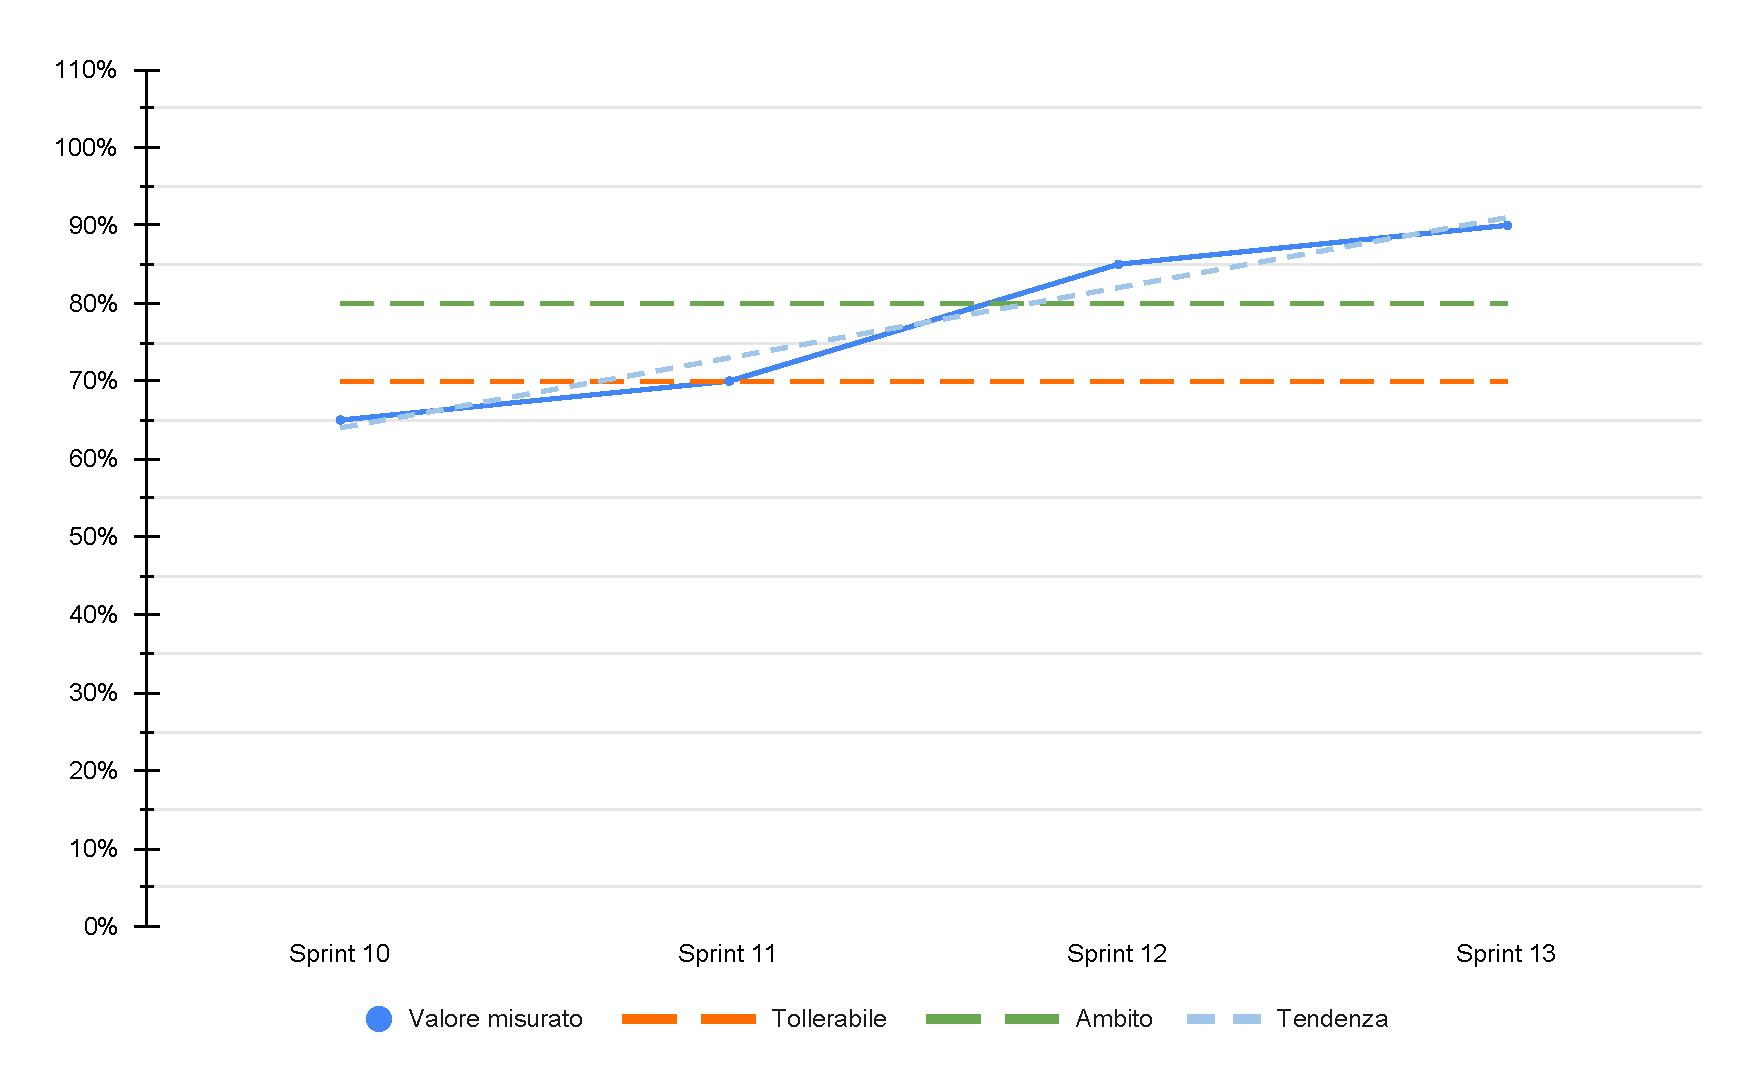
\includegraphics[width=\textwidth]{assets/rimozione_difetti.pdf}
  \caption{M.PD.18 - Rimozione dei difetti}
\end{figure}

\par Nel primo sprint della \glossario{PB}, il team ha configurato SonarCloud, uno strumento di analisi statica del codice finalizzato all'individuazione e alla rimozione dei difetti. A ogni aggiornamento di una \glossario{pull request}, il bot di SonarCloud genera un report che segnala potenziali problemi. L'obiettivo del gruppo era rimuovere tutti i difetti prima della chiusura delle pull request. Tuttavia, alcuni problemi di sicurezza e di affidabilità erano legati a Dockerfile o al template di PrimeVue. Pertanto, il team ha deciso di lasciare in sospeso la risoluzione di tali anomalie, assegnando loro un peso minore nel calcolo della metrica. A partire dallo \glossario{sprint} 12, l'implementazione dei test automatici e la configurazione di un workflow su \glossario{GitHub} hanno contribuito a ottimizzare il rilevamento dei difetti nel codice. Di conseguenza, la percentuale di rimozione dei difetti è salita progressivamente, superando il valore ambito. La maggior parte delle vulnerabilità rimosse riguardava la duplicazione del codice, che è stata ridotta significativamente. Nello sprint 12, il team ha corretto anche alcuni errori di sicurezza segnalati da SonarCloud.